\cotefile{162-5}

\cotefile{162-5}
\scanpage{25}
\[
\boxed{[X,dY]=\Theta_X(f)Y+f[X,Y]}\qquad\text{résulte de }\alpha
\]

Prouvons enfin la formule du crochet. Soit $\omega\in\Gamma\Omega$, on doit \deleted{vérifier} calculer
\[
\begin{aligned}
&\sum_{\substack{\text{perm.}\\\text{circ. sur}\\X,Y,Z}}
\bigl[-\langle\delta\omega,[X,Y]\wedge Z\rangle+\Theta_{[X,Y]}\langle\omega,\deleted{\unsure{Y}}Z\omega\rangle-\Theta_Z\deleted{\unsure{i_{[X,Y]}}}\langle\omega,[X\unsure{,}\,Y]\rangle\bigr]\\
={}&\sum\bigl[-\langle i_Z\delta\omega,[X,Y]\rangle+(\Theta_X\Theta_Y-\Theta_Y\Theta_X)\unsure{\langle}\omega,\deleted{\unsure{Y}}Z\rangle+\Theta_Z\langle\delta\omega,X\wedge Y\rangle\\
&\hspace{14em}-\Theta_Z\Theta_X\langle\omega,Y\rangle+\Theta_Z\Theta_Y\langle\omega,X\rangle\bigr]\\
={}&\sum-\langle i_Z\delta\omega,[X,Y]\rangle+\Theta_Z\langle\delta\omega,X\wedge Y\rangle\\
={}&\sum\langle\underset{\deleted{\unsure{\Theta_Z}}}{\delta i_Z}\delta\omega,X\wedge Y\rangle\,
\deleted{\unsure{+}}-\underset{\smash{\rule{.35pt}{2pt}\rule{9em}{.35pt}\rule{.35pt}{2pt}}}{\Theta_X i_Y\deleted{\delta}i_Z\delta\omega+\Theta_Y i_X i_Z\delta\omega}+\Theta_Z\langle\delta\omega,X\wedge Y\rangle\\
={}&\sum\bigl(i_X i_Y\underset{\inserted{\text{\textcircled{$\delta i_Z$}}}}{\deleted{\unsure{\delta i_Z}}}+\Theta_Z\deleted{\delta}i_X i_Y\deleted{\delta}\deleted{\unsure{+}}-\Theta_X i_Y i_Z+\Theta_Y i_X i_Z\bigr).(\delta\omega)
\end{aligned}
\]

\deleted{On va utiliser} $\deleted{\boxed{\Theta_{\unsure{Z|X}}=i_X\delta+\delta i_X}}$ \deleted{et les formules analogues en $Y,Z$, \unsure{pour trouver|qui donnent}}
\[
\begin{aligned}
&\deleted{\sum i_Y i_X\delta i_Z+i_Z\underset{\smash{\rule{.35pt}{2pt}\rule{1.4em}{.35pt}\rule{.35pt}{2pt}}}{\delta i_Y}i_X+\deleted{\unsure{\delta i_X i_Y i_X|\delta i_X i_Y i_Z}}}
\ \deleted{\overset{\inserted{\text{\unsure{permu|poser}}}}{\inserted{\delta i_Z i_Y i_X}}\unsure{-|=}i_X\underset{\smash{\rule{.35pt}{2pt}\rule{1.4em}{.35pt}\rule{.35pt}{2pt}}}{\delta i_Y}i_Z-\delta i_X i_Y i_Z}\\
&\hspace{12em}\deleted{\deleted{+}+i_Y\delta\underset{\smash{\rule{.35pt}{2pt}\rule{1.4em}{.35pt}\rule{.35pt}{2pt}}}{i_X i_Z}+\delta i_Y i_X i_Z}\\
&\deleted{\sum i_Y i_X\delta i_Z+(i_Z\delta i_Y i_X+i_Y\delta i_X i_Z\deleted{\unsure{+|\delta}}-i_X\delta i_Y i_Z)\unsure{-|=}3\delta i_X i_Y i_Z}\\
&\deleted{=-9\,\delta i_X i_Y i_Z+}
\end{aligned}
\]

On constate trivialement
\[
\begin{aligned}
&\sum-\Theta_X i_Y i_Z+\Theta_Y i_X i_Z=-2\sum\Theta_{\unsure{Z|X}}i_X i_Y\\
&\deleted{\sum\Theta_Z i_X i_Y=\unsure{-|+}\sum\Theta_X i_Y i_Z}
\end{aligned}
\]
donc on trouve
\[
\begin{aligned}
(\text{Jacobi})(\omega)&=T(\delta\omega),\quad\text{avec}\\
T&=\sum i_X i_Y\delta i_Z-\deleted{\unsure{\delta|i_Z}}\overset{\inserted{(\Theta_Z=i_Z\delta}}{\overset{\smash{\rule[-2pt]{.35pt}{2pt}\rule{2.4em}{.35pt}\rule[-2pt]{.35pt}{2pt}}}{\Theta_Z}}\,i_X i_Y\ \deleted{\unsure{=\frac{1}{2}i_{X\wedge Y}}}
\end{aligned}
\]
\margin{24}

\cotefile{162-5}
\scanpage{26}
Utilisons
\[
\boxed{\Theta_X\underset{\unsure{\triangleright}}{=}i_X\delta+\delta i_X}\quad\inserted{\text{(en degré quelconque)}}\quad\text{cf plus bas}
\]
il vient alors, au choix
\[
\begin{aligned}
T&=\sum i_X i_Y\delta i_Z-i_Z\delta i_X i_Y\deleted{\unsure{-\delta i_Z i_X i_Y}}\qquad \unsure{!|/}\quad\text{ou}\\
T(\delta\omega)&=\sum[i_{X\wedge Y},\Theta_Z](\delta\omega)
\end{aligned}
\]
\margin{pourquoi cela est-il nul ??}

On a donc une \uuline{$\Theta$-Algèbre de Lie} sur $X_0$, i.e. un \uline{Anneau de Lie} \deleted{sur} $\mathscr T$ sur $\deleted{\unsure{\underline O_{X_0}}}X_0$, muni d'un \uline{hom} \inserted{$\Theta:X\longmapsto\Theta_X$.} d'\uline{Anneaux} de Lie dans $\mathscr T_{X_0/\unsure{Z|\mathbb Z}}$, et d'une structure de $\underline O_{X_0}$-Module rendant $\Theta$ $\underline O_{X_0}$-linéaire et satisfaisant la formule $[\deleted{\unsure{\Theta}}X,fY]=\deleted{\unsure{f\Theta}}f[X,Y]+\Theta_X(f)Y$.

4.\quad \uline{Complexe de Cochaines associé à une $\Theta$-algèbre de Lie} \inserted{$\mathscr T$}

Cf. \unsure{mes notes|une note} Bourbaki ; on pose \deleted{(\unsure{supposant} qu'on soit sur un pt)}
\[
\underline{\unsure{C|\mathcal C}}^p=\underline{\mathrm{Hom}}(\bigwedge^p\mathscr T,O_{X_0})
\]
et on y définit une différentielle par une formule connue ..... .

Lorsque $\mathscr T$ provient d'un complexe de De Rham $(\bigwedge^*\Omega,\delta)$, alors l'hom d'alg. graduées évident $\bigwedge^*\Omega\longrightarrow C^*(\mathscr T)$ est \uline{compatible} avec les \deleted{structures} différentielles.

\margin{25}

\cotefile{162-5}
\scanpage{27}
5.\quad Les $\Theta$-Algèbres loc libres \inserted{de t.f. $\mathscr T$} sur $X_0$ correspondent exactement aux complexes de De-Rham sur $X_0$ construits sur des $\Omega$ loc. libres de t. f, par les correspondances de $3^\circ$. et $4^\circ$.

6.\quad Revenons au cas d'une catégorie formelle sur $X_0$, définie par $A=(A_\alpha)$ sur $X_0\deleted{\unsure{\mathcal C}}$\,...., et le complexe de De Rham associé $(\Omega^*\unsure{\underset{\nearrow}{=}|=}\bigwedge^*\Omega,\delta)$.

\uline{Th. de Quillen} \inserted{Supposons $X_0$ de car. nulle} Le foncteur $A\longmapsto(\Omega^*,\delta)$ induit une \uline{équivalence} entre la catégorie des catégories formelles \inserted{\unsure{adiques|-adiques}} sur $X_0$ dont le $\Omega\to$ \uline{plat}, et la catégorie des \deleted{Algèbres}\inserted{complexes} de De Rham $(\bigwedge^\alpha\Omega,\delta)$ sur $X_0$ dont le $\Omega$ \unsure{est|soit} \uuline{plat.} [Les $A$ en question ont la vertu que $\mathrm{Sym}\,\Omega\longrightarrow\mathrm{Gr}(A)$ est un isomorphisme, ce qui s'apparente \unsure{à|:} une propriété de ``lissité différentielle''.

Ceci contient le th. de Cartier sur les groupes formels en car. nulle.

Il y a une variante ``à puiss. divisées'', quand on met sur l'idéal d'augmentation de $A$ \inserted{$=(A_n)_{n\in\mathbb N}$} une structure d'\deleted{Algèbre} puiss divisées, qui passe au quotient sur les $A_n$, chaque $I_n$ étant nilpotent d'ordre $n$, et la filtration étant celle provenant des puiss. divisées. [À voir si dans cet énoncé il faut toujours des \unsure{relat.} entre la structure \deleted{\unsure{de}} puiss. divisées, \deleted{et} l'application $\Delta$ \ldots]

\margin{26}

\cotefile{162-5}
\scanpage{28}
7.\quad \uline{Coefficients} \inserted{\uline{sur catégorie formelle}} Soit $M$ un $\underline O_{X_0}$-module. La notion de ``donnée de descente'' sur $M$ relativement à $\mathcal C$ [ou ``$\mathcal C$-stratification'', ou ``opération de $\mathcal C$ sur $M$''] est claire. On constate alors \unsure{qu'une|que une} telle structure permet de mettre sur
\[
\bigwedge^*\Omega\otimes_{\underline O_{X_0}}M
\]
un opérateur différentiel $\delta_M$, tel que
\[
\begin{array}{l@{\qquad}l}
(*)&\delta_M(fx)=\delta(f)x\deleted{\unsure{\delta_M(x)}}+(-1)^{\deg F}f\,\delta_M(x).
\end{array}
\]
[Il suffit $=$ d'avoir une donnée de recollement d'ordre 1]

Un tel opérateur est connu quand on connait
\[
M\xrightarrow{\delta_M^1}\Omega\otimes M
\]
satisfaisant $(*)$ \deleted{\unsure{$\delta_M^1($}} pour $f\in\Gamma\underline O_{X_0}$ (donc $\deg f=0$).

\unsure{Le|La} fait que l'opérateur déduit \inserted{sur $\bigwedge^*\Omega\otimes M$ cf plus bas)} soit de carré nul provient de la condition de descente. [il suffit qu'elle soit vraie à l'ordre 2 \ldots??].

8.\quad \uline{Coefficients relatifs à une Algèbre de De Rham}

Plus gén, si $(\bigwedge^*\Omega,\delta)$ est une alg de De Rham sur $X_0$, on \deleted{\unsure{peut}} regarde les modules $M$ avec une \uline{connexion} relativement à celle-ci, i.e. un morphisme
\[
M\overset{\delta_M}{\mathbin{-}}\ \Omega\otimes M
\]
satisfaisant
\[
\delta_M(fx)=\delta(f)\otimes x+f\,\delta_M(x).
\]

\margin{27}

\cotefile{162-5}
\scanpage{29}
On peut alors de façon unique prolonger en une \deleted{dérivation} opération $\delta_M$ sur $\bigwedge^*\Omega\otimes M$, en posant
\[
\delta_M(\omega x)=\delta(\omega)\deleted{\unsure{\otimes}}x+\omega\,(\delta_M x)
\qquad\left(\begin{aligned}
&\omega\in\Gamma\bigwedge^*\Omega,\\
&x\in\Gamma\bigwedge^*\Omega\otimes M
\end{aligned}\right)
\]

Pour qu'on ait $\delta_M\delta_M=0$, il f. et s qu'on l'ait \deleted{\unsure{$\delta_M$}} en degré 0, i.e. que le composé
\[
M\xrightarrow{\delta_M^{\unsure{0|\bullet}}}\Omega\otimes M
\overset{\delta_M^1}{\mathbin{\unsure{-|\to}}}\bigwedge^2\Omega\otimes\deleted{\unsure{\wedge}} M
\]
soit nul. Ce composé s'appelle le \uline{tenseur} \uline{courbure}.

La donnée de \inserted{la connexion} $\delta_M^0$ permet de faire opérer $\mathscr T=\underline{\mathrm{Hom}}_{\underline O_X}(\Omega,\underline O_X)$ dans $M$, grâce.
\[
\Theta_X^M(x)=(X\otimes\mathrm{id}_M)(\delta_M^0(x))
\]
On a alors
\[
\begin{array}{r@{\ }l}
\begin{aligned}a)\\[1ex] b)\end{aligned}&
\left\{\begin{aligned}
\Theta_X^M(fx)&=\Theta_X(f)x+f\Theta_X^M(x)\\[1ex]
\Theta_{fX}^M(x)&=f\Theta_X^M(x)
\end{aligned}\right.
\end{array}
\]
D'autre part, si la connexion est sans \deleted{torsion}\inserted{courbure}, alors il est vrai \unsure{qu'on a|que}
\[
c)\quad\left\{\Theta^M_{[X,Y]}=[\Theta_X^{H},\Theta_Y^{H}].\right.
\]

\margin{28}

\cotefile{162-5}
\scanpage{30}
9.\quad \deleted{\unsure{Partant} d'une} \uline{Opération d'une $\Theta$.Alg. de Lie}

Soit $\mathscr T$ une $\Theta$-Algèbre de Lie sur $X_0$, $M$ un $\underline O_{X_0}$-Module. On dit que \deleted{$\mathscr T$} $M$ a une $\mathscr T$-connexion si on fait ``\unsure{opérer|operer}'' $\mathscr T$ sur $M$ de façon à satisfaire à a) et b) plus haut.

Ceci définit alors un tenseur courbure
\[
K\in C^2(\mathscr T,\mathrm{End}_{\underline O_{X_0}}(M))
\]
en posant
\[
K(X,Y)=\Theta_{[X,Y]}^M-\unsure{[|(}\Theta_X^M,\Theta_Y^H]
\]
Le tenseur courbure est donc nul ssi on a
\[
\Theta_{[X,Y]}^M=[\Theta_X^M,\Theta_Y^H],
\]
alors la connexion est \uline{dite intégrable}. Si $\mathscr T$ provient de $\Omega$ \inserted{$(\mathscr T=\underline{\mathrm{Hom}}_{\underline O_{X_0}}(\Omega,\underline O_{X_0}))$}, et $M$ \deleted{\unsure{provient}} muni d'une $\Omega$-connexion $\delta_M^0$, d'où un tenseur courbure
\diagram{\begin{tikzcd}[ampersand replacement=\&,column sep=large]
M\arrow[r]\arrow[rr,bend right=22,no head,"K'"'] \& \bigwedge^2\Omega\otimes M\arrow[r] \& C^2(\mathscr T,M)
\end{tikzcd}}
\unsure{si conventions|j'écris maintenant|j'aimerais}
\margin{Attention signes !}
\[
K(X,Y)(u)=K'(u)(X,X).
\]

\uline{10}.\quad Si \inserted{$(\bigwedge^*\Omega,\delta)$ avec défini\unsure{.}} $\Omega$ loc. libre de t.f. ($\Longleftrightarrow\mathscr T$ \inserted{$\Theta$-alg. de Lie sur $\mathscr T$} loc. libre de t.f.) alors pour un Module $M$ sur $\underline O_{X_0}$,

\margin{29}

\cotefile{162-5}
\scanpage{31}
les deux notions de connexion se correspondent biunivoquement, de $=$ que les deux notions de \inserted{tenseur courbure, de} connexion intégrable \ldots, et bien sur les complexes
\[
\bigwedge^*\Omega\otimes M\qquad\text{et}\qquad C^*(\mathscr T,M).
\]

11.\quad Sous les conditions du th de Quillen, ($X_0$ de car. nulle, \deleted{\unsure{la}} $(\bigwedge^*\Omega,\delta)$ \deleted{\unsure{loc. libre}}\inserted{avec $\Omega$ plat $\Leftarrow$} correspondant à une catégorie formelle $\mathcal C$ avec $\Omega$ plat, pour un Module $M$ sur $\underline O_{X_0}$, les structures de $C$-descente sur $M$ correspondent aux \deleted{\unsure{struct.}} $\Omega$-connexions sur $M$.

\margin{généralise mon th. fondamental de démarrage des cristaux\,\ldots. \unsure{Peut-il|Peut il} s'y ramener, en raisonnant dans un topos convenable ?!}

De plus, la cohomologie de De Rham de $M$, i.e $\mathbb H^{\unsure{\alpha|*}}(X,\bigwedge^{\unsure{\alpha|2|*}}\Omega\otimes M)$, est can. isom à la coh. de Hochschild (ou Čech-Alexander) de $C$ à coeff.\unsure{,|.|-} \unsure{dans|\deleted{dans}} $M$, plus précisément il y a un quasi-isom \inserted{canonique} de \inserted{complexes de} faisceaux abéliens (\unsure{dans 2 catég.|les 2 catég.} \unsure{dérivées|dérivée})
\[
\bigwedge^*\Omega\otimes M\simeq C^*(\mathcal C,M)
\]

\uline{Variante à puissances divisées}.

\margin{30}

\cotefile{162-5}
\scanpage{33}
\margin{notes du 10.9.68}

Tapis de Quillen.

I \quad \uline{Relations entre catégories et ensembles semi-simplic\deleted{\illegible{1}}a\deleted{\illegible{1}}ux}.

A toute catégorie $C$, on associe un ensemble semi-simpli\deleted{\unsure{v}}cial $S(C)$,
trouvant \deleted{\unsure{u}}a\deleted{n}insi un foncteur pleinement fidèle \deleted{de Cat}
\[ S;\ (\mathrm{Cat}) \longrightarrow (\mathrm{Ssimpl})\quad . \]
\deleted{Si C est associé à} Les systêmes locaux d'ensemble sur $SC$ correspondent
aux fancteurs sur $C$ qui transforment toute flêche en isomorphisme (i.e.
qu\deleted{\unsure{ç|t}}i se factorisent par le groupoïde associé à $C$). Les $H^i$ sur $SC$ d'un tel
systême local ($H^0$ pour ens, $H^1$ pour groupes, $H^i$ quelconques pour groupes
abéliens) s'interprètent en termes des foncteurs $\underleftarrow{\mathrm{lim}}^{(i)}$ déri\deleted{g}vés de $\underleftarrow{\mathrm{lim}}$ ,
ou si on préfère, des $H^i($ du \uline{topos} $C$ . On voit ainsi à quelle condition
un foncteur $C \to C'$ induit un\deleted{e} homotopisme $SC \to SC'$ : \deleted{i}en vertu du
critère cohomologique de Artin-Mazur, il f et s que pour tout systême
de coéfficients $F'$sur $C'$, l'homomorphisme naturel $\underset{C'}{\underleftarrow{\mathrm{lim}}}^{(i)}F' \longrightarrow \underset{C}{\underleftarrow{\mathrm{lim}}}^{(i\ )}F$
soit un isomorphisme (pour les i pour lesquels cela a un sens). \deleted{En termes}

A $C$ on peut asso\deleted{v}c\unsure{\deleted{i}e|\deleted{e}i}r le topos $\widetilde{C}$ , qui varie de façon \uline{covariante} avec $C$.
(NB le foncteur $C \mapsto \widetilde{C}$ n'a plus rien de pleinement fidèle, semble-t\deleted{\unsure{-}}il ??)
Les systêmes de coéfficients \inserted{ensemblistes} sur $C$ ( $\overset{\text{\inserted{déf}}}{=}$ les foncteurs \inserted{$C^o \longrightarrow \mathrm{Ens}$} transformant isomor-phismes en isomorphismes) correspondent aux faisceaux localement constant\deleted{,}s,
i.e. les objets localement constants de $\widetilde{C}$, définis intrinsèquement en termes
de $\widetilde{C}$ . Ainsi, le fait pour un foncteur $F:C \to C'$ d'induire un\deleted{e équivalence}
homotopisme $S(C) \to S(C')$ ne dépend que du morphisme de topos $\widetilde{F}: \widetilde{C} \to \widetilde{C'}$
induit, et signifie que pour tout faisceau localement constant $F'$ sur $C'$ i.
e. sur $\widetilde{C'}$ , les applications induites $H^i(\widetilde{C'},F') \longrightarrow H^i(\widetilde{C},\widetilde{F}^{*}(F'))$
sont des isomorphismes (pour les i pour lesquels cela a un\deleted{en} sens).

\margin{32}

\cotefile{162-5}
\scanpage{34}
On a aussi un foncteur évident
\[ T: (\mathrm{Ssimpl}) \longrightarrow (\mathrm{Cat}) , \]
en associant à tout ensemble semi-simplicial X la catégorie $T(X) = \Delta_{/X}$
des simplexes sur X, dont l'ensemble des objets est la réunion d\deleted{e}isjointe
des $X_n$ .... (c'est une catégorie fibrée sur la catégorie $\unsure{\Delta|\underline{\Delta}}$ des simplexes
types, à fibres les catégories discrètes définies par les $X_n$). Ceci posé,
Quillen prouve que pour tout X, ST(X) est isomorphe canoniquement à X dans
la catégorie homotopique construite avec (Ssimpl), et que pour toute C,
la catégorie TS(C) est \inserted{canoniquement} ``homotopiq\deleted{y}uement équivalente à C'' \deleted{dans le sens} i.e.
\inserted{\deleted{\unsure{à|è}}ca\deleted{\unsure{C}}noniquement} isomorphe à C dans la catégorie quotient de (Cat) obtenue en inversant les
foncteurs qui sont des homotopismes. \deleted{Il en résulte} Ces isomorphismes sont
fonctoriels en X. I\={l} en résulte formellement qu'un morphisme $f:X\to Y$ dans
(Ssimpl) est un homotopisme si et seulement si il en est ainsi de $T(f):T(X)$
$\to T(Y)$, d'où des foncteurs $S'$: $(\mathrm{Cat})' \longrightarrow (\mathrm{Ssimpl})'$ et $T'$:$(\mathrm{Ssimpl})'\longrightarrow(\mathrm{Cat})'$
entre les catégories ``homotopiques'', \inserted{construites avec (Cat) resp,(Ssimpl),} qui sont quasi-inverses l'un de l'aut-\\
re.

\deleted{\unsure{d}}De plus, Quillen construit un isomorphisme canonique et fonctoriel
dans (Cat)' entre C et la catégorie opposée $C^{\mathrm{o}}$ , ou ce qui revient au
m\deleted{\unsure{m}}ê\deleted{\unsure{e}}me, un isomorphisme canonique et fonctoriel dans (Ssimpl)' entre S(C) et
S($C^{\mathrm{o}}$). \deleted{Cela lui permet alors, pour} La définition est telle que le
foncteur induit sur les systêmes locaux sur C tra\deleted{\unsure{b|h}}ns\deleted{o}f\deleted{f}orme le foncteur
contrav\deleted{\unsure{r}}ariant F sur C, transformant t\deleted{\unsure{s|e}}oute flêche en flêche inversible, en
le foncteur covariant (i.e. contravariant sur $C^{\mathrm{o}}$) ayant mêmes valeurs sur
les objets, et obtenu sur les flêches en remplaçant F(u) par $F(u)^{-1}$; en
d'autres termes, l'effet de l'homotopisme de Quillen sur les group\deleted{i}oides
fondamentaux est l'isomorphisme évident entre les groupoides fondamentaux
de C et de $C^{\mathrm{o}}$ ,\deleted{qui est \unsure{l'ideni|l'idni}} compte tenu que le deuxième est l'opposé du

\margin{33}

\cotefile{162-5}
\scanpage{35}
premier. Comme applic\deleted{t}ation, Quillen obtient une interprétation faisceauti-
que de la cohomologie d'un ensemble semi-simplicial à coéfficients dans un
systême \inserted{local} con\deleted{tra}variant \inserted{$F$} \deleted{\unsure{de|dx}}(défini classiquement par le complexe cosimplicial
\margin{$\prod$ ?} des $C^n(F) = \rlap{\begin{tikzpicture}[overlay,x=1em,y=1em,baseline=0pt]\draw[black!35,line width=.3pt,rotate=25] (.40,-.20) ellipse (1.15 and .85);\end{tikzpicture}}\coprod\limits_{x\in X_n} F(x)$): on considère le systême local contravariant
défini par $F$, on l'interprète comme un faisceau sur \inserted{$T(X)$ i.e. objet de} $(\mathrm{Ssimpl})_{/X}$, et on
prend sa cohomologie. - Cependant, quand $F$ est un systême de coéfficien\unsure{\deleted{s}t|\deleted{t}s}s
cov\deleted{\unsure{r}}ariant pas nécessairement local, on n'a tjrs pas d'interp\unsure{\deleted{é}r|\deleted{r}é}étation de se\unsure{\deleted{n}s|\deleted{s}n}
groupes de cohomologie classiques en t ermes faisc\deleted{d}eautiques; ni, lorsque $F$
est co\deleted{\unsure{v}}n\deleted{a}tr\deleted{i}a\deleted{a}v\deleted{\unsure{n}}a\deleted{t}r\deleted{\unsure{,}}iant, de son homologie, ou inversement de sa cohomologie
faisceautique en termes classiques.

A propos de la notion de foncteur qui est un homotopisme. Quillen
montre qu\deleted{e}'un tel foncteur $F:C\longrightarrow C'$ induit une équiva\unsure{\deleted{n}l|\deleted{l}n}ence entre la sous-
catégorie triangulée \inserted{$D^b_{lc}(C')$} de la catégorie \inserted{dérivée \inserted{bornée} de celle \deleted{des}} des faisceaux abéliens sur $C'$, dont
les faisceaux de cohomologie sont des systêmes locaux, et la catégorie ana-
logue pour $C$; \deleted{Il s'en} et réciproquement. \deleted{Pour la partie directe} On peut
dans cet énoncé introduire aussi n'importe quel anneau de base (à condition
de le supposer $\neq 0$ dans le cas de la réciproque); \deleted{constant} la partie directe
vaut aussi avec un anneau de boefficients pas néc. constant, mais constant
tordu. Je pense que ce résultat (facile) doit pouvoir se généraliser ainsi:
Soit $f:X\quad X'$ un morphisme de topos qui soit tel que pour tout \deleted{systême}
faisceau loc. const. sur $X'$, $f$ induise un isomorphisme sur les cohomologies
(avec cas non commutatif inclus). Supposons que \deleted{\unsure{le} (\unsure{topos} $X$) soit} \inserted{$X$ et $X'$} \uline{localement}
\margin{
\begin{tikzpicture}[x=1em,y=1em,baseline=-.1em]\draw[line width=.65pt] (0,0) ellipse (.12 and .13);\draw[line width=.85pt] (.08,.1) .. controls (.20,.44) and (.44,.84) .. (.52,.99);\end{tikzpicture}} \margin{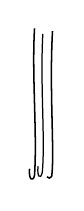
\begin{tikzpicture}[x=1em,y=1em]\draw[line width=.55pt] (0,5.5) .. controls (-.10,3.8) and (.10,1.7) .. (0,.20) .. controls (-.05,-.06) and (-.22,.02) .. (-.18,.43);\draw[line width=.45pt] (.30,5.3) .. controls (.20,3.5) and (.39,1.5) .. (.28,.29) .. controls (.21,.02) and (.08,.15) .. (.13,.52);\draw[line width=.55pt] (.65,5.4) .. controls (.53,3.3) and (.73,1.0) .. (.62,.15) .. controls (.58,.05) and (.49,.10) .. (.45,.14);\end{tikzpicture}} \uline{homotopiquement trivial}, i.e. que \deleted{tout} pour tout entier $n$\inserted{$\geq 1$}, tout objet $U$ \deleted{de}
\deleted{$X$}$'$ ait un \inserted{recouvrement} \deleted{revêtement} par des $U_i\longrightarrow U$, tels que a) tout systême local sur $U$
devient constant sur $U_i$, et toute section sur $U$ devient constante sur $U_i$,
et b) pour tout \deleted{systême} groupe abélien $G$, les $H^j(U,G)\unsure{\longrightarrow|\longleftrightarrow} H^j(U_i,G)$ sont
nuls pour $1\leq j\leq n$. Alors le foncteur $D^b_{lc}(X')\longrightarrow D^b_{lc}(X)$ induit par $f$ est

\figure{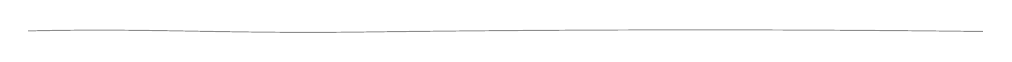
\begin{tikzpicture}[x=\linewidth,y=1em]\draw[black!45,line width=.35pt] (0,0) .. controls (.13,.10) and (.20,-.10) .. (.35,-.04) .. controls (.58,.06) and (.80,.06) .. (1,-.02);\end{tikzpicture}}

\margin{
\begin{tikzpicture}[x=1em,y=1em,baseline=-.1em]\draw[line width=.65pt] (0,0) ellipse (.12 and .13);\draw[line width=.85pt] (.08,.1) .. controls (.20,.44) and (.44,.84) .. (.52,.99);\end{tikzpicture} Attention, cette condition n'est typiquement \uline{pas} satisfaite par les schémas avec leur topologie étale (mais bien par \unsure{schémas} l. noeth. avec top. Zariski).}

\margin{34}

\cotefile{162-5}
\scanpage{36}

\deleted{pleinement fidèle (resp} une équivalence). Même énoncé si on met dans le
coup un \deleted{Anneau \unsure{loc}} systême local d'anneaux sur \(X'\).
E\unsure{\deleted{h}n|\deleted{n}h}fin, \(f\) induit \deleted{une}
\inserted{\deleted{foncteur pl fid (resp} une équivalence)}
\deleted{isomorphisme} entre la catégorie des coefficients locaux sur \(C\) et celle
des coéff. locaux sur \(C'\) \deleted{(?? peut-être cela doit il}
\inserted{\deleted{cette propriété doit}}\deleted{ être misedans les
hypothèses préliminaires sur \(f\) ?)} Principe de démonstration: on commence
par prouver ce dernier résultat, en notant que \deleted{dans le ca} si un topos est
loc\deleted{q}alement hom. trivial, il est loc\unsure{\deleted{a}.|a} connexe et loc. simplement connexe,
d'où une bonne théorie du \(\pi_o\) et du \(\pi_1\) (qui sont ici discrets), et on est
ra\(\unsure{\grave{m}|\overset{\inserted{n}}{m}}\)ené \deleted{pour} à un cas particulier du critère d'homotopisme de Artin et
Mazur, savoir un critère \inserted{cohomologique} pour qu'un homomorhisme de groupes \(G\longrightarrow H\) (ici \deleted{l}des
groupes \(\pi_1\) de \(X,X'\)) soit un isomorphisme: il doit induire des isomorphis\deleted{m}mes
sur les \(H^o\) et \(H^1\) (y inclus dans le cas non commutatif...). On prouve
la pleine fidélité en se ramenant par la suite spectrale aux cas \deleted{\unsure{t|l|e}}des \(\mathrm{Ext}^i\)
de coéfficients locaux. Par la suite spectrale encore, cela résultera du
fait suivant: si \(X^{\unsure{\deleted{\prime}|\prime}}\) est
\unsure{\deleted{h}lo\deleted{m}calement|\deleted{l}ho\deleted{c}malement} hom. trivial, alors la catégorie des
faisceaux abéliens loc. constants est stable par \(\underline{\mathrm{Ext}}^i\), et le foncteur
\(M\longmapsto M_X\) de\deleted{s faisceaux constants} (Ab) dans \(X_{ab}\) commute aux dits \(\mathrm{Ext}^i\).
En fait, \(X\) et \(X'\) étant loc homp\(\mid\)triviaux, les conditions suivantes sur \(f\)
seront équivalentes:

a) \(f\) est\unsure{b} un homotopisme, i.e. induit pour tout systême local (pas
néc commutatif) sur \(X'\)un isomorphisme sur les \(H^i\)\deleted{pour i \unsure{n|m}}.

b) \deleted{Même chose ave} \(f\) induit une équivalence \(D^b_{lc}(X')\longrightarrow D^b_{lc}(X)\).

\(a'\)) \(f\) induit une équivalence entre la catégorie des systêmes locaux
abéliens sur \(X'\) et \(X\), et des isomorphismes sur les \(H^i\) correspondants (donc
on ne prend ici que des coéfficients commutatifs).

\margin{?} J'ignore si on peut dans a) se borner aux sys\deleted{\unsure{y}}têmes locaux commutatifs,
\deleted{i\unsure{.}e\unsure{.} dans}
L'équivalence entre a) et b) fournit une première justification ou
motivation pour définir des types d'homotopie via la catégorie \(D^b_{lc}(X)\),

\margin{35}
\margin{\unsure{r}}

\cotefile{162-5}
\scanpage{37}
éventuellement muni de la sous-catégorie pleine de tous les systêmes locaux
sur X, et du foncteur cohomologique sur $D^b_{lc}(X)$ à valeurs dans lad\deleted{d}it\deleted{\unsure{u}}e
catégorie, et bien sûr du produit tensoriel (mais alors on sort de $D^b$
pour entrer dans $D^-$ , redactor demerdetur).

II n-catégories, catégories n-uples, et (Gr)-catégories.

Appelons bi-catégori\deleted{\unsure{i}}e une catégorie dans(Cat), i.e. un triple
$(C^{\deleted{o}}_{0},C^{\deleted{1}}_{1},$ \deleted{) où}$p_1,p_2,\pi$ ), où $C^o$ est une catégorie, $p_1,p_2$: $C^{\deleted{1}}_{1}\rightrightarrows C^{\deleted{o}}_{0}$ deux
foncteurs, $\pi:(C^{\deleted{1}}_{1},p_1)x_{C^o}(C^{\deleted{1}}_{1},p_2)\longrightarrow C^{\deleted{1}}_{1}$ un foncteur, avec les axiomes
habituels. Interprétant (Cat) comme la sous-catégorie pleine de (Ssimpl)
des objets qui .... , et de même pour les catégories à valeurs dans une
catégorie telle (Cat), on trouve que la catégorie \inserted{(Bicat)} des (Cat)-caté\deleted{t}gories
est équivalente à la sous-catégorie pleine de la catégorie des ensembles
bi-semisi\deleted{\unsure{p}}mplicia\deleted{y}ux

\[
\begin{array}{llll}
X^{\deleted{oo}}_{00} & X^{\deleted{\unsure{o1|d1}}}_{01} & \ldots & X^{\deleted{o,n}}_{0n}\\
X^{\deleted{1o}}_{10} & X^{\deleted{11}}_{11} & \ldots & X^{\deleted{1,n}}_{1n}\\
\multicolumn{4}{l}{\ldotp\;\ldotp\;\ldotp\;\ldotp\;\ldotp\;\ldotp\;\ldotp}
\end{array}
\]

formée des objets qui ligne par ligne et colonne par colonne satisfoht la
condition d'exctitude familière (transformer sommes amalgamées en produits
fibrés). De même la catégorie \deleted{des} (Tricat) des (Bicat)-catégories
\unsure{\deleted{'}s\deleted{s}'}interprète en t ermes d'objets tri-\inserted{semi}simpliciaux, etc.

Exemple: soit C une catégorie, posons $C^{\deleted{o}}_{0}=C$, $C^{\deleted{1}}_{1}=\underline{\mathrm{Fl}}(C)$, avec structures
$p_1,p_2$, évidentes (d'où une (Cat)-catétorie dont les composantes semi-sim-\\
pliciales supérieures sont les catégories $\underline{\mathrm{Fl}}^n(C)$ des n-flêches de C ...).
L'ensemble bi-semisimplicial correspondant a pour composantes les ensembles
$\mathrm{Hom}(\Delta^n x\Delta^m,C)$. Par exemple, les objets de $X^{\deleted{11}}_{11}$ sont les carrés commutatifs
de flêches de C, qu'on peut interpréter(de deux manières différentes) comme

\margin{36}

\cotefile{162-5}
\scanpage{38}

morphismes de flêches.

Notons une symmétrie évidente dans la c atégorie (Bicat), interprétée
en termes d\deleted{e}'ensemble bi-semisimpliciaux, obtenue en échangeant les lignes
et les colonnes dans \deleted{les} de tels ensembles bi... \deleted{q}Un ensemble bisemisimplic\unsure{i}\linebreak
al qui ... peut donc de deux façons différentes être consi\deleted{\unsure{i}}déré comme défi-\linebreak
nissant une bicatégorie. De même le groupe symétrique $\mathrm{Sym}_n$ opère sur
la catégorie \deleted{de} (n-upcat) des catégories n-uples ..

Une 2-catégorie peut être définie comme const\unsure{\deleted{t}i}\unsure{\deleted{u}t}\unsure{\deleted{t}u}ée par un ensemble
\deleted{discret} $C^{\deleted{o}}_0$ (l'ensemble des objets ), qu'on interprètera comme une catégo\linebreak
rie discrète, plus la donnée pour tout $x,y \in C^{\deleted{o}}_0$ d'une catégorie $\underline{\mathrm{Hom}}(x,y)$,
plus \inserted{des foncteurs} \deleted{une} composition entre celles\deleted{(}-ci ... Prenant la catégorie somme \deleted{de} $C^{\deleted{1}}_1$
des $\underline{\mathrm{Hom}}(x,y)$, On peut exprimer la donnée de ces foncteurs de composition,
et des sources et buts \inserted{$x,y$} dans les catégories $\underline{\deleted{\unsure{\mathrm{C}|\mathrm{O}}}\mathrm{Hom}}(x,y)$, comme définis par
des foncteurs ``sou\deleted{c}rce'' et ``but'' $C^{\deleted{1}}_1 \to C^{\deleted{o}}_0$, et un foncteur de composition
$C^{\deleted{1}}_1 \mathrm{x}_{C^{\deleted{o}}_0} C^{\deleted{1}}_1 \longrightarrow C^{\deleted{1}}_1$ , les axiomes des 2-catégories correspondant exactement aux
axiomes des(Cat)-catégories. De cette façon, la catégorie des 2-catégories
est équivalente à la catégorie des (Cat)-catégories qui ont une ``catégorie
d'objets'' qui est discrète, ou encore à la catégorie des Bicatégories
qui, interprétées comme ensembles bi-semisimpliciaux, ont \deleted{une} comme
première ligne un ensemble \unsure{\deleted{b}s}emi\unsure{\deleted{e}s|\deleted{o}s}\unsure{\deleted{s}i}\unsure{\deleted{i}m}plicial discret (i.e. un foncteur cons-\linebreak
tant sur $\Delta$ ). Il parait qu'on a une interprétation simple dans le même
esprit de la notion de n-catégorie en termes d'ensembles n-semi-simpliciaux

\margin{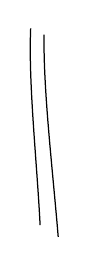
\begin{tikzpicture}[x=1mm,y=1mm,baseline=(current bounding box.north)]
\draw[line width=.45pt] (0,0) .. controls (-.3,-7) and (.8,-17) .. (1.2,-25);
\draw[line width=.45pt] (1.7,-.8) .. controls (1.6,-8) and (2.8,-18) .. (3.5,-26.5);
\end{tikzpicture}}
\deleted{ou} Demander à Quillen relations entre la notion de m-\deleted{\unsure{c|e}}Catégorie dans
la catégorie (n-Cat), et celle de ensemble (m+n)-semisimplicial.\linebreak
\deleted{(en particulier entre cette dernière notion et celle de}

L'interprétation standard semisimpliciale permet d'interpréter

\margin{37}

\cotefile{162-5}
\scanpage{39}
\figure{\begin{tikzpicture}[x=1cm,y=1cm]\draw[line width=.45pt] (0,.9) -- (0,.18) .. controls (1.8,.1) and (2.3,.18) .. (3,.08) .. controls (5,-.12) and (6.2,.07) .. (7,.02) -- (7.15,.28) -- (9,.18);\end{tikzpicture}}

\margin{\unsure{!} Attention : la catégorie $\underline{\mathrm{Hom}}_{\mathrm{grab}}$, qui s'identitifie à la catégorie definie par un $R\mathrm{Hom}_{Z}(C_x,C'_x)$; ce point devant être élucidé!}

de même les (Cat)-groupes(ou groupes à valeurs dans (Cat)) comme étant
les groupes semisimpliciaux qui ``sont''des catégories i.e. qui \deleted{se défini\unsure{\deleted{d}s|d}-}
\deleted{s\unsure{e|o}nt} satsifont la condition d'exactitude familière, \deleted{i}permettant d'en déterminer
tous les composants à l'aide de $C_o$\deleted{$_{\unsure{u|a}}$} et $C_1$ . Appliquant le tapis de
Dold, dans le cas commutatif, on trouve que les (Cat)-groupes abéliens
forment une catégorie équivalente à celle des complexes de chaines de
groupes abéliens qui sont de longueur 1:
\[
0 \leftarrow C_o \leftarrow C_1 \leftarrow 0 \quad .
\]
Quand on explicite l\unsure{\deleted{e}a|\deleted{a}e} (Cat)-groupe abélien associé à un tel complexe de
chaines, on trouve ``ma'' construction chérie d\unsure{\deleted{a}e|\deleted{e}a} la ``catégorie de Picard''
associée au complexe: objets ceux de $C_o$ , flêches de $x$ dans $y$ les $z$ dans $C_1$
tels que $dz=y-x$ . On trouve donc à isomorphisme ppès tous les groupes
abéliens de (Cat) ainsi. Un \uline{complément important} est que toute catégorie
de Picard \inserted{\deleted{(resp. et}} \deleted{commutative)}est équivalente (au sens technique qu'on ne précise
pas ici) à \deleted{la catégorie} un vrai (Cat)-groupe \inserted{\deleted{(resp. (Cat)-groupe}} \deleted{commutatif)} .
\inserted{Quand on \unsure{simplifie} mod ``\unsure{Grab}'' équivalence, cela correspond à travailler dans la \uline{catégorie} \uline{dérivée} des complexes Seuls invariants sont $H_0\,H_1$ (\unsure{qui jouent|ou l'invariant} $\unsure{\Pi|\pi}_0\,\unsure{\Pi|\pi}_1$)}
\margin{\deleted{\unsure{Quillen dit} mais cela contredit les résultats de \unsure{Verdier} \unsure{la fin} \unsure{de} \illegible{1}}}
\margin{Mais \unsure{attention|alors} si on part d'une ``cat. de Picard commut.'', elle ne se réalise que par un (Cat)-g. \uuline{non} \uline{comm.}}

On notera qu'on a une \deleted{\unsure{interp}} classification beaucoup plus restreinte
que pour les H-espaces (resp. les H-espaces homotopiquement comm.) mod
équivalence d'homotopie, de façon précise entre les groupes resp. les grou-
pes abéliens de la catégorie homotopique. La raison en est qu\inserted{'}on est beau\deleted{co}coup
plus restrictif dans le contexte catégorique pour le sens d\unsure{\deleted{a}e|\deleted{e}a} l'associativité
(resp. et de la commutativité), puisqu'on ne demande pas seulement
l'existence d'isomorphismes d'associ\deleted{\unsure{i}}a\deleted{i}tivité\deleted{,} (qui suffirait pour avoir un
groupe dans \inserted{la catégorie homotopique} $(\mathrm{Cat})' \approxeq (\mathrm{Ssimpl})'$, modulo l'existence d'unités et d'inverse)
mais qu'on suppose \uline{donné\deleted{e}s} ces isomorphismes, de façon à satisfaire à cer-
taines compatibilités: c'est ce qui permet, me semble-t-il, de prouver qu'à
\margin{\deleted{\uuline{\unsure{pas vrai|pourquoi}}}} \margin{(} équivalence près, on peut supposer qu'il s'agit de vrais groupes dans
(Cat), \deleted{resp. de vraie commutativité.}

\margin{38}

\cotefile{162-5}
\scanpage{40}

On doit trouver une approximation meilleure d'un cran à la classifica
tion topologique en prenant des (2-Cat)-groupes resp. des (2-Cat)-groupes
abéliens, ou plus généralement des ``Gr-2\unsure{'}-catégories'' resp.
``G\unsure{\deleted{a}r\deleted{r}a|\deleted{r}a\deleted{a}r}b-2-catégories'' . (NB U\deleted{n}ne Grab-catégorie défi\deleted{\unsure{t|n}}nit une Grab-2catégorie
comme une catégorie définit une 2-catégorie; du point de vue semi-simplici-
al, cette opération serait analogue à celle de ``cosquélette\deleted{''} tronqué'';
Mais également une Grab-2-catégorie définie en G\unsure{\deleted{R}r|\deleted{r}R}ab-catégorie\deleted{\unsure{.}}, savoir la
catégorie des automorphismes de l'objet unité; cette \deleted{dé} opération serait
analogue à celle de ``tuage des groupes d'homotopie en dim $>1$''). Pour la
notion gro\deleted{i}ssière (Gr\deleted{\unsure{ab}} ou Grab) l'idée de ma lettre à Verdier était qu'o\unsure{n}
doit trouver la même chose que les tronqués\inserted{au cran 2}, dans la catégorie \uline{homotopique}
des H-espaces - i.e. ce qu'on d\unsure{\deleted{d}é|\deleted{é}d}duit des H-espaces par tuage des groupes
d'homotopie en dimensions $>2$.

\margin{\figure{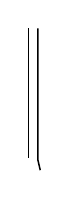
\begin{tikzpicture}[x=1cm,y=1cm,line width=.55pt]
\draw (0,0) -- (0,-1.65);
\draw (.12,0) -- (.12,-1.67) -- (.15,-1.80);
\end{tikzpicture}}}
(Demander à Quillen relations exactes entre \deleted{H}o\deleted{\unsure{-}}bjets-groupes et objets
\deleted{ponctués} connexes de la catégorie homotopique\inserted{ponctuée}: forment-ils des catégories équivalen-
tes par le foncteur espace des lacets?).
\margin{non, on a un foncteur pl. fidèle (?) mais pas \unsure{ess.$^t$|ess.} surjectif .....}

Pour les \uline{vrais} groupes\inserted{abéliens} de (2-Cat), l'approche de Quillen consiste à
les identifier \deleted{à}d'abord à des groupes abéliens de la catégorie \deleted{\unsure{d}}(Bicat),
donc à des gr\unsure{\deleted{p}o|\deleted{o}p}upes abéliens bi-semi\deleted{e}simpliciaux particuliers (\unsure{ć|c}onditions
sur chaque ligne et chaque colonne). Appliquant la version bi-semisimplici
ale du tapis de Dold, on trouve que \deleted{cette ca} la catégorie de ces objets
estb équivalente à la catégorie des \deleted{objets} bicomplexes\inserted{de chaines} de groupes abéliens
qui sont nuls en dehors du carré $\unsure{\deleted{1}0|\deleted{0}1}\leq i,j\leq1$. \deleted{Quillen dit que} La co\unsure{\deleted{o}l|\deleted{l}o}onne
que la première ligne corresponde à un \deleted{ensemble} groupe semisimplicial
trivial signifie alors qu'elle n'a que le terme de degré zéro, i.e. que
le bicomplexe est réduit à

\diagram{\begin{tikzcd}[ampersand replacement=\&,column sep=2.8em,row sep=2.2em,
execute at end picture={
\node[anchor=east,inner sep=0pt] (extraForty) at ([xshift=-.08em]lowerForty.west) {$\unsure{\deleted{0}|\theta}$};
\node[anchor=north,inner sep=0pt] (clippedForty) at ([xshift=-.65em,yshift=-.08em]lowerForty.south) {$\unsure{\pi_2}$};
\draw (extraForty.south) .. controls +(-.18,-.26) and +(-.22,0) .. (clippedForty.west);
}]
C_{oo} \& 0 \arrow[l] \& 0 \arrow[l] \\
|[alias=lowerForty]| C_{1o} \arrow[u] \& C_{11} \arrow[l] \arrow[u] \& 0 \arrow[l]
\end{tikzcd}}

\margin{39}

\cotefile{162-5}
\scanpage{41}
\unsure{\deleted{L}C}\unsure{\deleted{a}e}s\deleted{e} bicomplexes s'identifient aux complexes de c\unsure{\deleted{a}h}\unsure{\deleted{h}a}ines de lo\unsure{\deleted{g}n}\unsure{\deleted{n}g}ueur 2.\linebreak
Donc la catégorie de (2-Cat)-groupes abéliens est équivelente à celle des\linebreak
complexes de chaines de longueur 2. L'explicitation de la 2-catégorie\linebreak
associée à un tel complexe de chaines est mon interprétation chérie. Il\linebreak
faudrait encore expliciter l\unsure{\deleted{e}a}\deleted{s morphismes} 2-Grab-catégorie des\linebreak
homomorphismes (en un sens à préciser) entre deu\unsure{\deleted{t}x}\deleted{el} tel\unsure{\deleted{s}l}es 2-Grab-catégo-\linebreak
ries strictes, en termes d'un complexe $\mathrm{RHom}$.

L'idée qui se dégage de cette approche, et que Quillen on espère va\linebreak
expl\unsure{\deleted{o}i}citer, c'est que la \deleted{notion de catégorie de} notion\deleted{s} de groupe abélien\linebreak
dans (n-Cat) correspond à celle de complexe de \inserted{chaines de} longueur n, en raisonnant\linebreak
soit mod. isomorphisme de part et d'autre, soit mod. une notion naturelle\linebreak
de n-équivalence d'un côté, et dans la catégorie dérivée de l'autre. Ceci\linebreak
doit pouvoir se préciser en utilisant des $\mathrm{Hom}^{\bullet}$ resp. des $\mathrm{RHom}^{\bullet}$.

Si maintenant C est une catégorie avec un ``produit tensoriel'' associa\linebreak
tif (et éventuellement unitaire), i.e. un bifoncteur avec des isomorphis-\linebreak
mes d'associativité (mais sans inverse ...), on peut lui associer \unsure{\deleted{(}s}ans\linebreak
doute une Gr-catégorie universelle (tout comme à un monoïde on associe un\linebreak
groupe symmétrisé), d'où des invariants, qu'on pourra désigner par $K_o(C)$\linebreak
et $K_1(C)$. On suppose qu'on pourra de même trouver, pour tout n, une\linebreak
Gr-n-catégorie universelle où envoyer C de façon compatib\unsure{\deleted{o}l|\deleted{b}l}e avec $\otimes$ (\unsure{\deleted{d}t}out\linebreak
cela dans un sens à préciser), dont les invariants $\pi_n$ seraient par défini\linebreak
tion les $K_n(C)$. \unsure{\deleted{E}U}\unsure{\deleted{e}n} cas intéressant est celui où C est une catégorie avec\linebreak
produits finis (par exemple une catégorie additive) et $\otimes$ est le produit\unsure{;|,}\linebreak
\deleted{mais} \deleted{(}\inserted{[}Mais on notera que dans le cas d'une catégorie non seulement additive\linebreak
mais abélienne, il y a une notion plus adéquate du $K_o$, qui devrait corres\linebreak
pondre à une notion plus adéquate de la suite des $K_i$, inspirée du tapis\linebreak
de Roos; sans doute c'est en termes de (``vraie'') catégories triangulées

\margin{40}

\cotefile{162-5}
\scanpage{42}
qu'i\unsure{\deleted{o}l} conviendra de poser les définitions adéquates). - Peut-être Quillen\linebreak
\margin{\uuline{oui}} \margin{\figure{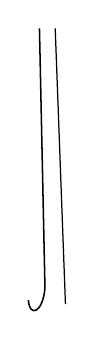
\begin{tikzpicture}[x=1cm,y=1cm]\draw[line width=.55pt] (0,3.5) -- (.07,.20) .. controls (.04,-.12) and (-.13,-.17) .. (-.14,.05);\draw[line width=.45pt] (.20,3.5) -- (.33,0);\end{tikzpicture}}}a-t-il une définition semi-si\unsure{\deleted{p}m}pliciale plus directe, sans passer par des\linebreak
n-catégories, des $K_i$ et plus précisément du H-espace qui devrait correspon-\linebreak
dre à C. \deleted{Dans le cas} Ce n'est certainement pas \inserted{en général} l'ensemble semi-simplicial\linebreak
SC \deleted{engendré à} associé à C, puisque dans le cas d'une catégorie additive,\linebreak
C est homotopiquement trivial (en effet le foncteur identique est ``homotope\linebreak
au foncteur nul, puisqu'il suffit d'avoir un homomorphisme d'un foncteur\linebreak
dans l'autre; d'où une équivalence d'homotopie entre C et la catégorie\linebreak
nulle). Pourtant, il semble bien que dans le cas où C est une Gr-catégorie\linebreak
\margin{\unsure{$\xi$|$\zeta$}} \margin{\figure{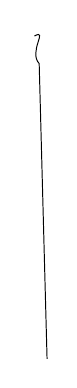
\begin{tikzpicture}[x=1cm,y=1cm]\draw[line width=.35pt] (0,4.1) .. controls (.18,4.2) and (-.08,3.9) .. (.06,3.75) -- (.16,0);\end{tikzpicture}}}i.e. admet des inverses, alors ce soit bien la construction ``naïve'' SC qui\linebreak
est la bonne, puisqu'on trouve bien un $\pi_o$ et un $\pi_1$ qui sont aussi les\linebreak
$\pi_o$ et $\pi_1$ au sens catégorie sans Gr-structure.

\margin{À expliquer : pour des Gr-n-catégories, les $\pi_i$ au sens\linebreak
\unsure{$\xi$|$\zeta$} \figure{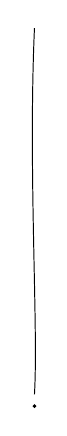
\begin{tikzpicture}[x=1cm,y=1cm]\draw[line width=.35pt] (0,4.8) .. controls (-.08,3) and (.05,1) .. (0,.15);\fill (0,0) circle (.025);\end{tikzpicture}} semi-simplicial sont aussi les $\pi_i$ au sens Gr-n-catégories,\linebreak
savoir les objets à isom près dans divers $\underline{\mathrm{Hom}}(1,1)$ ...... \deleted{Il y a\linebreak
aussi une interprétation de l'opération \unsure{$\Omega$ : espace des lacets}\linebreak
en termes d'opération \unsure{du|de} shift géométrique évidente sur les\linebreak
n-catégories .....}}

\margin{41}

\cotefile{162-5}
\scanpage{43}

\margin{42}

\cotefile{162-5}
\scanpage{44}
III   Point de vue ``motivique'' en théorie du cobordisme.

Soit C la catégorie des variétés différe\unsure{\deleted{b}n|\deleted{n}b}tiables (pas nécessairement
ori\unsure{\deleted{n}e|\deleted{a}e}\unsure{\deleted{b}n|\deleted{b}e}tables), \inserted{les morphismes étant les classes d'homo\unsure{\deleted{o}t|\deleted{t}o}opie d'applications continues.} Si B est une catégorie, on s'intéresse aux couples
$(F_{.},F^{\cdot})$ d'un foncteur covariant et d'un foncteur contravariant de C
dans B, satisfaisant les conditions que pour tout $X\in\mathrm{Ob}\,C$, on a $F_{.}(X)=$
$F^{\cdot}(X)$, et que si on a un produit fibré ordinaire
\diagram{
\begin{tikzcd}[ampersand replacement=\&,column sep=small, row sep=small]
 \& X' \arrow[dl, "g'"'] \arrow[dr, "f'"] \& \\
X \arrow[dr, "f"'] \& \& Y' \arrow[dl, "g"] \\
 \& Y \&
\end{tikzcd}
},
avec f et g transversaux, alors on a $g^{\cdot}f_{.} = f'_{.}g'^{\cdot}$ \inserted{(on pose $f_{.}=F_{.}(f),f^{\cdot}=F^{\cdot}(f)$\unsure{)}}. La question est
de trouver une B et un couple $(F_{.},F^{\cdot})$ qui soient ``universels'' dans un
sens évident. Quillen prouve que la construction suivante donne une
telle solution.

Pour toute variété $X\in\mathrm{ob}\,C$, on définit un anneau commutatif
$B(X)$ (l'anneau de bordisme de X) en prenant comme éléments les classes
\deleted{de} d'éléments de C au dessus de X, pour la relation de cobordisme:
$f':X'\to X$ et $f'':X''\to X$ sont équivalents, s'il existe une variété à bord
Z, et un $f:Z\to X$, tel que bord $Z = X'\amalg X''$ et $f'$ et $f''$ sont induits
par f. La somme de $B(X)$ est la somme disjointe (c'est une loi de groupe,
\deleted{l'inverse étant} où tout élément est d'ordre \deleted{1}\inserted{2} \deleted{\unsure{ou 2}}), le produit est
donné par le produit fibré, en utilisant le théorème de trabsversalité
de Thom pour bouger un peu $f''$, de sorte à le rendre transversal à $f'$.
\inserted{\uline{NB} L'anneau est de plus \uline{gradué} par la dimension relative ....}
Si on a $f: X\to Y$, on définit $f_{.} : B(X)\to B(Y)$ de façon évidente (toute
variété sur X est sur Y), et $f^{\cdot}: B(Y)\to B(X)$ par produit fibré (utili\unsure{\deleted{(}-|(-}
sant encore le th. de transversalité). De cette façon, $B(X)$ devient un
foncteur-anneau \inserted{(gradué)} contravariant en X, et un foncteur groupe covariant en

\margin{43}

\cotefile{162-5}
\scanpage{45}

$X$. De plus, on a la formule \inserted{du type $g^{\cdot}f. = f'.g'^{\cdot}$ ci-dessus, impliquant \unsure{la|le} \unsure{formule|formules}} de projection habituelle. Ceci posé, les
constructions bien connues en théorie des correspondances permettent
de définir une catégorie $\underline{B}$ dont l\unsure{\deleted{d}e|\deleted{e}d}s objets sont ceux de $C$, et les
Hom étant donnés par
\[
\mathrm{Hom}_{B}(X,Y) = B(XxY) \quad .
\]
On a un isomorphisme canonique $\underline{B} \simeq \underline{B}^{o}$, qui est l'identité sur les
objets et la symmétrie $B(XxY)\simeq B(YxX)$ sur les flêches, et un foncteur
évident \deleted{$\unsure{B|C}\quad\underline{B}$} $F. : C \to \underline{B}$, qui est l'identité sur les objets et donné
par les graphes sur les flêches. Composé avec la symmétrie précédente,
on trouve un foncteur $F^{\cdot}$: \deleted{$B$\unsure{(}} $C \relbar \underline{B}$. On vérifie enfin que le couple
$(F.,F^{\cdot})$ satisfait aux conditions envisagées dans l'alinéa 1 (ceci aussi
devrait être formalisé au cas des correspondances générales ...). \deleted{\unsure{I}}O\deleted{\unsure{l}}n
vérifie enfin qu'il a la propriété universelle qu'il faut. Lorsqu'on
se donne un couple $(F'.,F'^{\cdot})$ à val eursdans une catégorie $B'$, il faut
trouver une factorisation par $B$. Elle est toute trouvée sur les
objets, il faut la définir sur les flêches, donc définir, pour $X,Y$
dans $C$, une application
\[
\begin{array}{ll}
(*) & \qquad B(XxY) \to \mathrm{Hom}(X',Y') \quad .
\end{array}
\]
Mais si $Z$ est au\deleted{d}dessus de $XxY$, d'où $p:Z\to X$ et $q:Z\to Y$, on lui associe
un élément du deuxième membre de (*) comme le composé
\[
X' \overset{F'^{\cdot}(p)}{\longrightarrow} Z' \overset{F'.(\unsure{\deleted{p}q|\deleted{q}p})}{\longrightarrow} Y' \quad .
\]
Il faut prouver que l'élément obtenu en remp\unsure{\deleted{l}a|\deleted{a}l}çant $Z$ \inserted{$=Z_0$} par un $Z_1$ cobor\deleted{d}
dant au dessus de $X$ \inserted{est le même}. Or si $g:T\to XxY$ réalise le cobordisme, on
voit (regardant seulement $T$ et la décomposition $\mathrm{bord}(T) = Z_0\amalg Z_1$)
qu'il existe une variété $\overline{T}$ sur $S^1$ (obtenue en ``doublant'' $T$) \deleted{et une}
\deleted{application $T$ \unsure{une}} transversale au dessus d'un couple de poi\unsure{\deleted{h}n|\deleted{n}h}ts $s_o,s_1$
de $S^1$, tels que $Z_i$ soit l'image inverse \inserted{dan\unsure{s} $\overline{T}$} de $s_i$ ($i=0,1$); d'autre part,

\margin{44}

\cotefile{162-5}
\scanpage{46}
$g$ manifestement se prolonge en $\overline{g} : \overline{T} \to X\mathrm{x}Y$ . Cela nous ramène à prouver
que \inserted{le composé} $\unsure{F'}\overline{T}' \xrightarrow{\alpha_i} \unsure{F'}Z'_i \xrightarrow{\alpha_{i*}} \unsure{F'}\overline{T}'$ ne dépend pas de $i=0,1$. Ecrivons $X$ au lieu de $\overline{T}'$,et
considérons le diagramme cartésien d'inclusions
\diagram{\begin{tikzcd}[ampersand replacement=\&]
X_s \arrow[r, "\alpha_s"] \arrow[d, "\alpha_s"'] \& X \arrow[d, "{\Gamma \unsure{\overset{\Delta}{=}|=} (p,\mathrm{id}_X)}"] \\
X \arrow[r, "i_s"] \& S^1\mathrm{x}X
\end{tikzcd}}
,

on a alors $\alpha_s^*\alpha_{s*}=\Gamma^*i_{s*}$ , qui ne dépend pas de $s$ puisque $i_s$ n'en
dépend pas à homotopie près. - Le reste est sans doute l'AQT.

Sur la strcture des $B.(X)$. Ce sont tous des algèbres graduées
sur $B.(\mathrm{pt})=\Lambda$ , qui est une algèbre graduée à degrés positifs, réduite
\margin{\unsure{\S}}
à $\underline{F}_2$ en degré\deleted{s} 0. C'est d'ailleurs une algèbre de polynômes \inserted{à une infinité de générateurs
$x_i$ ($i$ entier $\unsure{\geq|>}1$\unsure{,} $\neq$ de la forme $2^\nu-1$)} connue ...
\inserted{d'ann\unsure{\deleted{a}e}\unsure{\deleted{d}a}\unsure{\deleted{x}u}xp\unsure{\deleted{d}g}\unsure{\deleted{i}r}\unsure{\deleted{e}a}\unsure{\deleted{e}d}ués}
On a un homomorphisme évident $B.(X)\to H^{\unsure{\deleted{P}L|\deleted{L}P}}(X)$, nul en degrés $>$0, qui
à tout $Z$ sur $X$ associe l'image de $1\in H^o(Z)$ par l'homomorphisme de Gysin
associé à $Z\to X$. Cet homomorphisme par Thom est surjectif (toute clas-%
\margin{en fait $H^\bullet(X)\simeq B.(X)/\Lambda^+B.(X)$}
se de cohomologie provient d'une image de variété compacte ...); \deleted{noter}
On ppouve même qu'il existe un relèvement fonctoriel en $X$
\margin{?}
$H^\bullet(X)\to B.(X)$, (\inserted{il est douteux qu'il soit} compatible avec multiplication) \deleted{tel}tel que l'on ait:

\deleted{a)}\unsure{1)} L'homomorphisme correspondant $H^\bullet(X)\otimes_{\underline{F}_2}\Lambda\simeq B.(X)$ est un iso-%
\margin{?}
morphisme (ce sera vrai pour tout relèvement individuellement ...), \deleted{et}

\deleted{b)}2) [\inserted{Quillen ignore si} \deleted{Le}le relèvement est compatible aussi avec les hom. de Gysin.]

Ainsi, la catégorie $\underline{B}$ admet un foncteur pleinement fidèle dans la
catégorie des modules gradués libres de type fini sur $\Lambda$, les modules
de type fini qu'on obtient ainsi ayant des générateurs à degrés $<$ 0 et
satisfaisant (pour $X$ connexe i.e. quand il y a un seul générateur de
degré zéro) la dualité de Poincaré. Quand on prend la catég\unsure{\deleted{b}o|\deleted{o}b}rie quasi-%
abélienne-\inserted{$\unsure{\widetilde{B}|B}$}associée à $\underline{B}$, on trouve donc tous les modules gradués libres
de type fini à générateurs \deleted{négatifs} en degrés $\leq$ 0 seulement. C'est une

\margin{45}
